\documentclass{article}
\usepackage[margin=1in]{geometry}
\usepackage{problemset}
\showsolntrue

% Custom commands
\newcommand{\R}{\mathbb{R}}
\newcommand{\X}{\mathcal{X}}
\newcommand{\Y}{\mathcal{Y}}
\newcommand{\E}{\mathbb{E}}
\newcommand{\V}{\text{Var}}
\renewcommand{\P}{\mathbb{P}}
\newcommand{\x}{\mathbf{x}}
\newcommand{\w}{\mathbf{w}}

\begin{document}
\pstitle{%
    COGS 181A%
}{
    Homework 1%
}[due Tuesday, January 13 at 11:59PM]

\begin{probset}
\begin{prob}[\textbf{(10 points) Conceptual Questions}]
    Assume we have a binary classification model:
    \[ f(x) = \begin{cases}
        +1, & \text{if } \w \cdot \x + b \geq 0 \\
        -1, & \text{if } \w \cdot \x + b < 0
    \end{cases} \]
    where the feature vector $\x = (x_1, x_2) \in \R^2$, bias $b \in \R$, weight vector $\w = (w_1, w_2) \in \R^2$.
    The decision boundary of the classification model is:
    $\w \cdot \x + b = 0$

    \begin{subprobset}
        \begin{subprob}
            If the predictions of the classifier $f$ and its decision boundary $\w \cdot \x + b = 0$ are shown in Figure 1, which one below can be a possible solution of weight vector $\w$ and bias $b$?
            \begin{enumerate}[label=\Alph*.]
                \item $\w = (+1, 0), b = -1$.
                \item $\w = (-1, 0), b = +1$.
                \item $\w = (+1, 0), b = +1$.
                \item $\w = (0, -1), b = -1$.
            \end{enumerate}

            \begin{figure}[H]
                \centering
                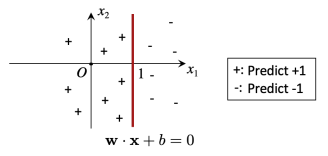
\includegraphics[width=0.5\textwidth]{Images/fig1.png}
                \caption{Decision Boundary 1}
            \end{figure}

            \begin{soln}
                \textbf{B}: $\w = (-1, 0), b = +1$.
            \end{soln}
        \end{subprob}

        \newpage

        \begin{subprob}
            If the predictions of the classifier $f$ and its decision boundary $\w \cdot \x + b = 0$ are shown in Figure 2, which one below can be a possible solution of weight vector $\w$ and bias $b$?
            \begin{enumerate}[label=\Alph*.]
                \item $\w = (+1, 0), b = -1$.
                \item $\w = (-1, 0), b = +1$.
                \item $\w = (+1, 0), b = +1$.
                \item $\w = (0, -1), b = -1$.
            \end{enumerate}

            \begin{figure}[H]
                \centering
                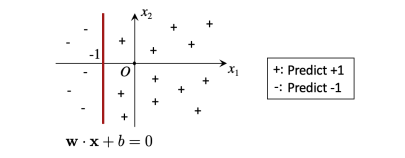
\includegraphics[width=0.6\textwidth]{Images/fig2.png}
                \caption{Decision Boundary 2}
            \end{figure}

            \begin{soln}
                \textbf{C}: $\w = (+1, 0), b = +1$.
            \end{soln}
        \end{subprob}
    \end{subprobset}
\end{prob}

\begin{prob}[\textbf{(15 points) Decision Boundary}]
    \begin{subprobset}
        \begin{subprob}
            \textbf{(5 points)} We are given a classifier that performs classification in $\R^2$ (the space of data points with 2 features $(x_1, x_2)$) with the following decision rule:
            \[ h(x_1, x_2) = \begin{cases}
                +1, & \text{if } x_1 + 2x_2 - 4 \geq 0 \\
                -1, & \text{otherwise}
            \end{cases} \]
            Draw the decision boundary of the classifier and shade the region where the classifier predicts $1$. Make sure you have marked the $x_1$ and $x_2$ axes and the intercepts on those axes.

            \begin{soln}
                The shaded region is the region where the classifier predicts $1$, the unshaded region is the region where the classifier predicts $-1$. The intercepts are $(4, 0)$ and $(0, 2)$.
                \begin{center}
                    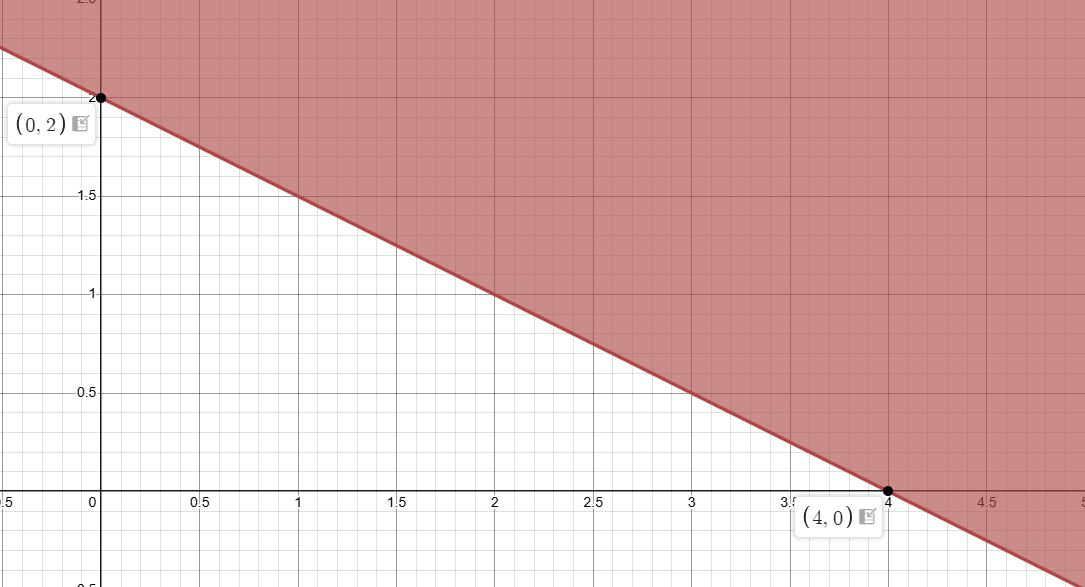
\includegraphics[width=0.6\textwidth]{Images/2.1.png}
                \end{center}
            \end{soln}
        \end{subprob}

        \newpage

        \begin{subprob}
            \textbf{(10 points)} We are given a classifier that performs classification on $\R^2$ (the space of data points with 2 features $(x_1, x_2)$) with the following decision rule:
            \[ h(x_1, x_2) = \begin{cases}
                +1, & \text{if } w_1x_1 + w_2x_2 + b \geq 0 \\
                -1, & \text{otherwise}
            \end{cases} \]
            Here, the normal vector $\w$ of the decision boundary is normalized, i.e.:
            \[ \|\w\|_2 = \sqrt{w_1^2 + w_2^2} = 1. \]

            \begin{enumerate}
                \item Compute the parameters $w_1, w_2$ and $b$ for the decision boundary in Figure 3. Please make sure the predictions from the obtained classifier are consistent with Figure 3.
                
                \textbf{Hint:} Please use the intercepts in the Figure 3 to find the relation between $w_1, w_2$ and $b$. Then, substitute it into the normalization constraint to solve for parameters.

                \item Use parameters from the above question to compute predictions for the following two data points: $A = (3, 2)$, $B = (-1, 0)$.

                \begin{figure}[H]
                    \centering
                    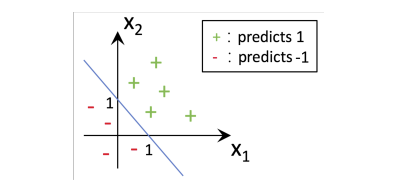
\includegraphics[width=0.5\textwidth]{Images/fig3.png}
                    \caption{Decision Boundary to solve for parameters}
                \end{figure}
            \end{enumerate}

            \begin{soln}
                \begin{enumerate}
                    \item The line is $x_2 + x_1 - 1 = 0$. Therefore, $w_1 = w_2 = -b$. Since $\|\w\|_2 = 1$ and plugging in (0, 0) yields a negative value, we have $w_1 = w_2 = \frac{1}{\sqrt{2}}$ and $b = -\frac{1}{\sqrt{2}}$.
                    \item The predictions for the data points $A = (3, 2)$ and $B = (-1, 0)$ are $1$ and $-1$ respectively.
                \end{enumerate}
            \end{soln}
        \end{subprob}
    \end{subprobset}
\end{prob}

\newpage

\begin{prob}[\textbf{(15 points) One Hot Encoding}]
    A dataset $S$ is denoted as $S = \{\x_1, \x_2, \x_3, \x_4, \x_5\}$, where each sample refers to the specification of a cellphone.

    \begin{center}
        \begin{tabular}{c|||c|c|c|c}
            & Height (mm) & Width (mm) & Make & Color \\
            \hline
            $\x_1$ & 144 & 71 & Apple & Gold \\
            $\x_2$ & 162 & 76 & Samsung & Silver \\
            $\x_3$ & 150 & 70 & Samsung & Black \\
            $\x_4$ & 149 & 71 & Google & Silver \\
            $\x_5$ & 158 & 78 & Apple & Black \\
            \hline
        \end{tabular}
    \end{center}

    Represent this dataset $S$ using a matrix and briefly explain your design decisions.

    \textbf{Hint:} (1) For the categorical feature, you may use the one-hot encoding strategy. (2) You may choose either a row vector or a column vector to represent each data sample in your result. If you use a row vector to represent each data sample, the shape of the result matrix should be $5 \times 8$.

    \begin{soln}
        \[ S = \begin{bmatrix} 144 & 71 & 0 & 0 & 0 & 0 \\ 162 & 76 & 1 & 0 & 1 & 0 \\ 150 & 70 & 1 & 0 & 0 & 1 \\ 149 & 71 & 0 & 1 & 1 & 0 \\ 158 & 78 & 0 & 0 & 0 & 1 \end{bmatrix} \]
        The first two columns are the height and width of the cellphone. The next four columns are the one-hot encoding of the make and color of the cellphone. Since there are 3 values for each categorical feature, only need 2 columns for each feature since all 0s can encode one value. In this case, if the third and fourth columns are both 0, then the make is Apple. If the last two columns are both 0, then the color is Gold. Similarly, column 3 is for Samsung, column 4 is for Google, column 5 is for Silver, and column 6 is for Black.
    \end{soln}
\end{prob}

\begin{prob}[\textbf{(10 points) Vector Projection}]
    For each pair of vectors, compute the cosine similarity:
    \begin{subprobset}
        \begin{subprob}
            $\begin{bmatrix} 4 \\ -5 \\ 3 \end{bmatrix}$ and $\begin{bmatrix} 4 \\ 5 \\ 3 \end{bmatrix}$

            \begin{soln}
                \[\cos \theta = \frac{16 - 25 + 9}{\sqrt{4^2 + (-5)^2 + 3^2} \sqrt{4^2 + 5^2 + 3^2}} = \frac{0}{50} = 0\]

                Therefore, the cosine similarity is 0 since the vectors are orthogonal.
            \end{soln}
        \end{subprob}

        \begin{subprob}
            $\begin{bmatrix} -1 \\ 1 \\ -1 \end{bmatrix}$ and $\begin{bmatrix} 1 \\ -1 \\ -1 \end{bmatrix}$

            \begin{soln}
                \[\cos \theta = \frac{-1 - 1 + 1}{\sqrt{(-1)^2 + 1^2 + (-1)^2} \sqrt{1^2 + (-1)^2 + (-1)^2}} = \frac{-1}{3}\]

                Therefore, the cosine similarity is $-\frac{1}{3}$.
            \end{soln}
        \end{subprob}
    \end{subprobset}
\end{prob}
\end{probset}
\end{document}